\documentclass[12pt, openany]{report}
\usepackage[utf8]{inputenc}
\usepackage[T1]{fontenc}
\usepackage{amsmath,amsfonts,amssymb}
\usepackage{amssymb}
\usepackage{multicol}
\usepackage[a4paper,left=2.5cm,right=2.5cm,top=2.5cm,bottom=2.5cm]{geometry}
\usepackage[french]{babel}
\usepackage{libertine}
\usepackage{graphicx}
\usepackage{wrapfig}
\usepackage{float}
\usepackage{enumitem}
\usepackage{pythonhighlight}
\usepackage[]{titletoc}
\usepackage{empheq}
\usepackage{titlesec}
\usepackage{mathpazo}
\usepackage{xfrac}
\usepackage{textcomp}
\usepackage{mathtools}
\usepackage{caption}
\usepackage{tabularray}
\usepackage{subcaption}
\usepackage[bottom]{footmisc}
\usepackage{pdfpages}
\usepackage{tabularx}
\usepackage[skins]{tcolorbox}
\titleformat{\chapter}[display]
  {\normalfont\bfseries}{}{0pt}{\Huge}
\usepackage{hyperref}
\newcommand{\hsp}{\hspace{20pt}}
\newcommand{\HRule}{\rule{\linewidth}{0.5mm}}
\newcommand\independent{\protect\mathpalette{\protect\independenT}{\perp}}
\def\independenT#1#2{\mathrel{\rlap{$#1#2$}\mkern2mu{#1#2}}}

% Define a new tcolorbox style with a red border and transparent interior
\tcbset{
    redbox/.style={
        enhanced,
        colframe=red,
        colback=white,
        boxrule=1pt,
        sharp corners,
        before skip=10pt,
        after skip=10pt,
        box align=center,
        width=\linewidth-2pt, % Adjust the width dynamically
    }
}
\newcommand{\boxedeq}[1]{
\begin{tcolorbox}[redbox]
    \begin{align}
        #1
    \end{align}
\end{tcolorbox}
}

\begin{document}


\begin{titlepage}
    \begin{sffamily}
    \begin{center}
        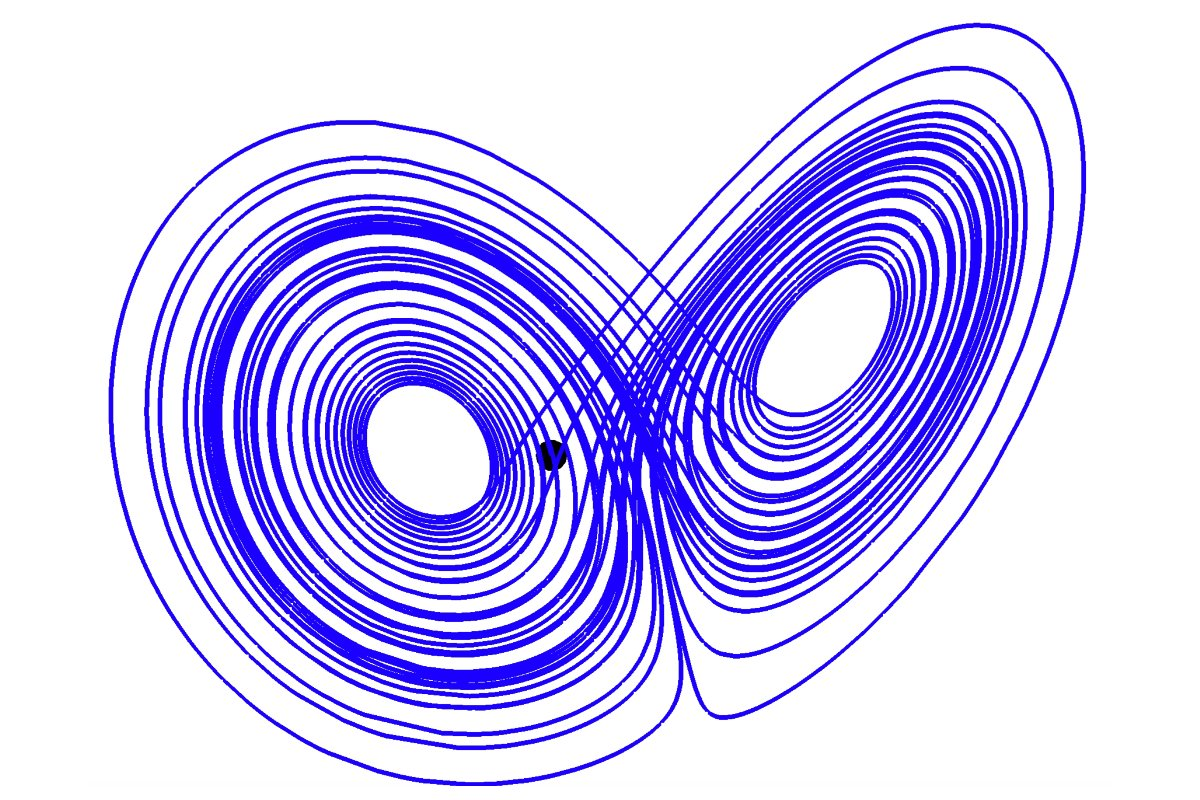
\includegraphics[scale=0.25]{img/page_de_garde.png} \\[1cm]
        \HRule \\[0.4cm]
        { \huge \bfseries LINMA2171 Numerical Analysis \\[0.4cm] }
    
        \HRule \\[1.5cm]
        \textsc{\LARGE Simon Desmidt}\\[1cm]
        \vfill
        \vspace{2cm}
        {\large Academic year 2024-2025 - Q1}
        \vspace{0.4cm}
         
        
\includegraphics[width=0.15\textwidth]{img/epl.png}
        
        UCLouvain\\
    
    \end{center}
    \end{sffamily}
\end{titlepage}

\setcounter{tocdepth}{1}
\tableofcontents
\chapter{Linear continuous-time 2D dynamical systems}
\section{Introduction}
Consider the 2D dynamical system \(\dot x=f(x),\: x\in \mathbb{R}^n\). Let \(\Omega \subseteq \mathbb{R}^n\) that is compact and positively invariant. Assume that \(f\in \mathcal{C}^1\) on \(\Omega\), i.e. it is continuously differentiable on \(\Omega\). Let \(x(0)\in \Omega\). Then the system has one and only one solution for all positive times. \\

\(\Omega\) is positively invariant if \(x(0)\in \Omega\Longrightarrow x(t)\in \Omega \: \forall t\ge 0\). 
\section{General form}
The general form of a linear dynamical system is 
\begin{equation}
    \dot x=Ax \qquad x\in \mathbb{R}^n
\end{equation}
and its solution is of the form \(x(t) = \exp(At)x(0)\). We will now study the different possibilities of stability, based on the matrix \(A\):
\begin{enumerate}
    \item \(A\) is diagonalizable:
    \begin{enumerate}
        \item \(\lambda_1>\lambda_2>0\) : unstable (repelling) node (see LINMA2370).
        \item \(\lambda_1>\lambda_2=0\) : 
        \item \(\lambda_1>0>\lambda_2\) : saddle point.
        \item \(0=\lambda_1>\lambda_2\) : 
        \item \(0>\lambda_1>\lambda_2\) : attracting node.
        \item \(\lambda_1=\lambda_2>0\) : unstable star, the eigenvectors are perpendicular and the direction is repelling from the origin.
        \item \(\lambda_1=\lambda_2=0\) : every point is an equilibrium.
        \item \(\lambda_1=\lambda_2<0\) : stable star, the eigenvectors are perpendicular and the direction is going to the origin.
    \end{enumerate}
    \item \(A\) has two equal eigenvalues with only one eigenvector, i.e. is not diagonalizable:
    \begin{enumerate}
        \item \(\lambda<0\): convergence to the equilibrium point.
        \item \(\lambda=0\): 
        \item \(\lambda>0\):
    \end{enumerate}
    \item \(A\) has complex conjugate eigenvalues:
    \begin{enumerate}
        \item \(Re(\lambda)>0\): diverges from the equilibrium in a spiral form.
        \item \(Re(\lambda)=0\): the trajectory is periodic, does not converge nor diverge.
        \item \(Re(\lambda)<0\): converges to the equilibrium in a spiral form.
    \end{enumerate}
\end{enumerate}

\end{document}